\chapter{JDart et exécution concolique}
	\paragraph{}
		L'idée générale est de rendre la tâche de tester des Applets Java Card moins penible et plus la plus efficace possible.
		Pour cela nous optons pour l'utilisation de l'exécution concolique comme une technique d'analyse, ce qui permet de rendre 
		le système à tester moins obscur et plus prédictible. Surtout quand on est face à des systèmes complexes
		nécessitant des méthodes plus avancées qu'un simple test unitaire.
    
	\paragraph{}
		\textbf{JDart \footnote{JDart : https://github.com/psycopaths/jdart}} est un outil qui permet d'utiliser l'exécution concolique
		comme une technique de tests pour les applications Java.
		\newline
		Il se présente sous forme d'une extension de \gls{JPF} un outil créé par la NASA afin de tester ses applications, y compris les programmes executés sur ses robots astromobiles.
	\section{Exploration des chemins et l'exécution concolique}
		\subsection{Java Path Finder: Exploration des chemins}
			\nocite{JPF}
			
			\paragraph{}
				\gls{JPF} est un outil de vérification des modèles d'états pour le bytecode Java,
				en réalité \gls{JPF} est une \gls{VM} qui exécute le programme donné en entrée autant de fois que nécessaire
				afin d'explorer chaque chemin qu'il contient.
				
				Tout au long de ce processus, \gls{JPF} collecte les anomalies rencontrées telles que l'interblocage des threads et les exceptions non traitées, puis il génére un rapport contenant les traces qui ménent à ces anomalies.
	
			\begin{figure}[H]
				\centering
					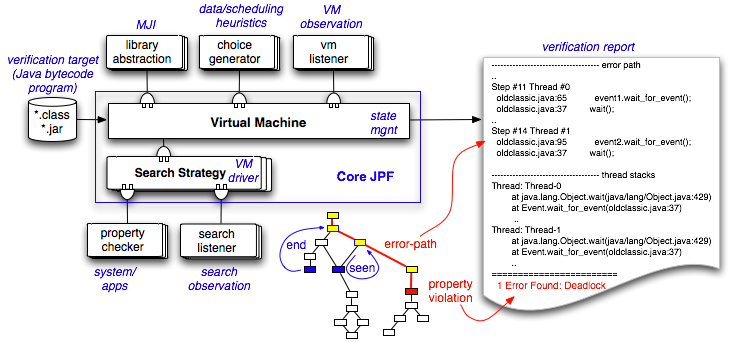
\includegraphics[scale=0.5]{images/jpf-model.png}
				\caption{Modèle d'opération de \gls{JPF}}
			\end{figure}
	
			\paragraph{}
				\gls{JPF} ne se limite pas simplement à détecter les erreurs d'un programme, en effet, il effectue la vérification des modéles.
				C'est un outil qui permet de simuler le non-determinisme. Certain aspects ne peuvent pas être contrôlés par de simples tests et exigent l'assistance d'une \gls{VM}.
				Cependant, en essayant d'explorer et exécuter tous les chemins au sein d'un programme, le nombre d'executions nécessaires peut croître d'une maniére exponentielle (On parle du problème d'explosion d'état). 
				Pour résoudre ce problème, \gls{JPF} réalise une correspondance d'état, c'est un mecanisme qui permet de comparer
				l'état actuel en un n\oe{}ud à des états déjà connus, dans le cas où l'état
				a été verifié \gls{JPF} est capable d'effectuer un retour arrière à la position précédente la plus proche où un chemin inexploré existe et restaure l'état du programme à tester à cette position.
	
			\begin{figure}[H]
				\centering
					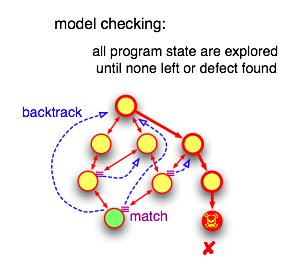
\includegraphics[scale=0.5]{images/jpf-model-checking.png}
				\caption{Vérification du modéles}
			\end{figure}
      
			\paragraph{}
				La vérification des modèles (\textit{Model Checking}) ne dépend pas des conjectures. En théorie si une anomalie est présente dans le programme à tester
				alors la vérification des modéles la trouvera, puisque c'est une méthode qui explore de maniére exhaustive tous les comportements possibles du systeme ;
				d'où vient l'efficacité du \textit{Model Checking}.
		\subsection{JDart: Exécution concolique}
			\nocite{JDart}
			\nocite{JDart2}

			\paragraph{}
				\gls{JPF} n'est pas une boite noire. L'une des meilleures fonctionalités de \gls{JPF} est la possibilité de le personnaliser entièrement et d'ainsi pouvoir ajouter des extensions facilement.
				Cet aspect a permi la création d'un grand nombre d'extensions utiles comme des moteurs
				qui permettent l'exécution symbolique et concolique.

			\paragraph{}
				Une execution concolique commence par une entrée concrète, en exécutant le programme à tester, des contraintes symboliques pour les chemins explorés
				sont formés pour cette exécution. Ces contraintes symboliques sont en réalité des formules logiques composés d'un tas de déclarations conditionnelles
				qui ont été collecté tout au long du parcours.

				L'étape suivante consiste à nier une sous formule et donc nous arrivons à créer un nouveau vecteur de valeurs concrétes en utilisant un
				solveur de contraintes.

				Ce vecteur sera utilisé pour une nouvelle exécution du programme qui permettra d'éxplorer un nouveau chemin.
				Cette procedure peut être répéter jusqu'à ce que tous les chemins possibles du système à tester sont explorés.
				
			\begin{figure}[H]
				\centering
					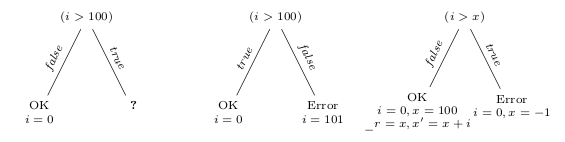
\includegraphics[scale=0.5]{images/concolic.png}
				\caption{Exécution concolique}
			\end{figure}
				
			\paragraph{}
				L'execution concolique résout un grand problème qui occure généralement au cours de l'exécution concolique,
				puisque l'espace de recherche est réduit significativement de façon à ce que le problème d'explosion d'espace de recherche
				ne peut plus se réaliser car les formules logiques générées par l'execution symbolique indiquera quelle valeur concrète
				doit être fournie pour satisfaire la condition concernée.
				Il n'est plus obligatoire de fournir un grand nombre d'entrée qui au final peuvent générer toutes un même chemin.
				\newline
				La technique d'exécution concolique a aussi son effet sur l'exécution symbolique traditionnelle.
				En effet, quand une condition ne peut pas être résolue symboliquement à cause de la complexité de la contrainte (Equation mathématique complexe,
				opération sur les nombres flottant...) elle sera remplacer par une valeur concréte ce qui permet de continuer l'exploration des chemins.

			\paragraph{}
				JDart est l'une des extensions de \gls{JPF}, il s'agit d'un moteur d'exécution concolique qui traite un programme Java
				en utilisant à la fois des valeurs symboliques et concrétes garde les traces des exécution symboliques.
				Les formules logiques créées sont ensuite passées à un solveur \textit{\gls{SMT}} afin d'obtenir une évaluation satisfaisante de la contrainte.
				JDart utilise par défaut \textit{\gls{microsoft-z3}} mais aussi il propose un niveau d'abstraction qui permet d'intégrer d'autres solveurs
				si nécessaire tels que: \textit{Coral}, \textit{dreal}...
				
			\begin{figure}[H]
				\centering
					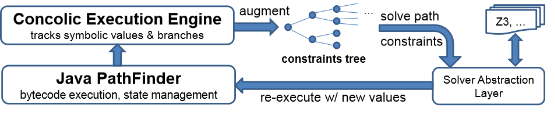
\includegraphics[scale=0.5]{images/archJDart.png}
				\caption{Architecture de JDart}
			\end{figure}
				
      
	\section{La VM JAVA, la VM du JPF et la VM JavaCard}
	\section{Tester des applets JavaCard}
	\paragraph{}
		Java Path Finder est connu comme le couteau suisse de la vérification Java,
		il est en effet un des outils de test les plus evolués pour les applications Java,
		notamment grâce à son extensibilité et à son habilité à supporter et intérger de nouvelle extensions.
		Cependant, la majorité des extensions ne sont pas destinées à être executées sur des systèmes JavaCard.